\begin{table}[htbp]\centering\small
\caption{Paired capacity-scenario summaries on 100 disturbance tapes.}
\label{tab:funded_controls}
\begin{tabular*}{\textwidth}{@{\extracolsep{\fill}}lrrrr@{}}
\toprule
Regime & \shortstack{Constraint\\hit (\%)} & \shortstack{Composite\\event (\%)} & \shortstack{Mean\\dislocation} & \shortstack{Min. equity\\(\$)} \\
\midrule
Active memory & 100.0 & 100.0 & 1.76570 & 9999.06 \\
Frozen memory & 100.0 & 100.0 & 1.15086 & 9999.06 \\
Zero feedback & 100.0 & 100.0 & 1.12686 & 9997.99 \\
Inventory limit removed & 0.0 & 100.0 & 5.06952 & -122.03 \\
\bottomrule\end{tabular*}
\par\smallskip\begin{minipage}{\textwidth}\footnotesize Dislocation is the time-average absolute displacement over 64 steps, in dollars. The hit flag is not a permanent trading ban: subsequent reversing fills remain possible. Removing the inventory limit does not add funding. Means are descriptive; these summaries do not include uncertainty for each arm mean.\end{minipage}
\end{table}
\begin{table}[htbp]\centering\small
\caption{Paired dislocation contrasts (dollars).}
\label{tab:funded_paired_contrasts}
\begin{tabular*}{\textwidth}{@{\extracolsep{\fill}}lrr@{}}
\toprule
Contrast & Mean difference & Paired bootstrap 95\% interval \\
\midrule
Active minus frozen & 0.61484 & [0.61477, 0.61490] \\
Active minus zero feedback & 0.63884 & [0.63871, 0.63897] \\
\bottomrule\end{tabular*}
\par\smallskip\begin{minipage}{\textwidth}\footnotesize Percentile intervals use 1,000 resamples of paired tapes. They describe this fixed simulation, not real-market intervention effects or a universal variance-reduction guarantee.\end{minipage}
\end{table}
\begin{figure}[htbp]\centering
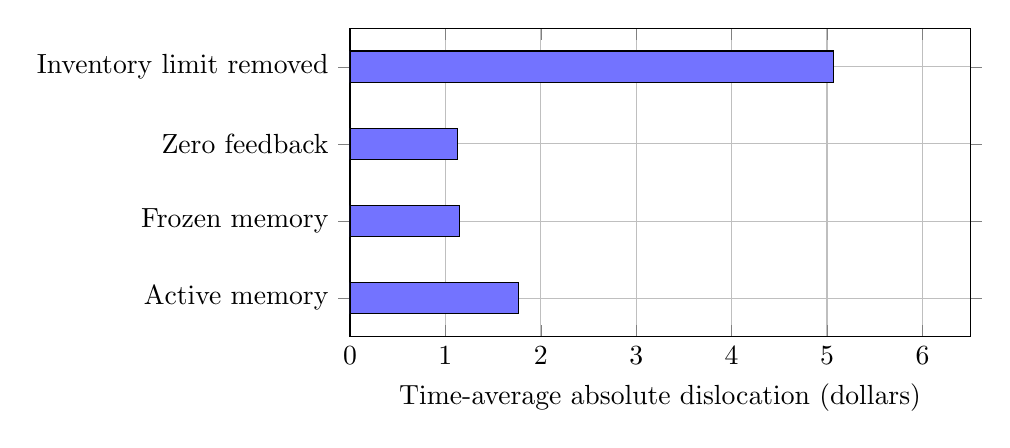
\begin{tikzpicture}\begin{axis}[width=.78\textwidth,height=5.5cm,xbar,
xmin=0,xmax=6.5,ymin=.5,ymax=4.5,ytick={1,2,3,4},
yticklabels={Active memory,Frozen memory,Zero feedback,Inventory limit removed},
xlabel={Time-average absolute dislocation (dollars)},grid=major]
\addplot[fill=blue!55,draw=black,bar width=.4cm] coordinates {(1.7657007,1) (1.1508616,2) (1.1268573,3) (5.0695227,4)};
\end{axis}\end{tikzpicture}
\caption{Descriptive regime means, generated from the preserved scenario rules.
Paired-difference uncertainty is reported separately in
Table~\ref{tab:funded_paired_contrasts}. The unconstrained adaptive transition
has spectral radius $1.07409$, so this is not a stable-system
safety counterexample.}\label{fig:paired_mechanism_dislocation}\end{figure}
